\normaltrue
\correctionfalse

%\UPSTIidClasse{11} % 11 sup, 12 spé
%\newcommand{\UPSTIidClasse}{11}


\exer{Mouvement TT -- $\star$ \label{C1:05:03}}
\setcounter{numques}{0}
\UPSTIcompetence[2]{B2-14}
\UPSTIcompetence[2]{B2-15}
\UPSTIcompetence[2]{C1-05}
\index{Compétence B2-14}
\index{Compétence B2-15}
\index{Compétence C1-05}
\index{Torseur des actions mécaniques transmissibles}
\index{Torseur d’une action mécanique extérieure}
\index{Principe fondamental de la statique}
\index{PFS}
\index{Mécanisme à 2 translations}
\ifcorrection
\else
\textbf{Pas de corrigé pour cet exercice.}
\fi

\ifprof
\else
Soit le mécanisme suivant. On note $\vect{AB}=\lambda(t)\vect{i_0}$ et $\vect{BC}=\mu(t)\vect{j_0}$.
$G_1 = B$ désigne le centre d'inertie de \textbf{1},et $m_1$ sa masse. %et $\inertie{G_1}{1}=\matinertie{A_1}{B_1}{C_1}{0}{0}{0}{\bas{1}}$; 
$G_2 = C$ désigne le centre d'inertie de \textbf{2} et  $m_2$ sa masse. % et $\inertie{G_2}{2}=\matinertie{A_2}{B_2}{C_2}{0}{0}{0}{\bas{2}}$.

 Un vérin électrique positionné entre \textbf{0} et \textbf{1} permet de maintenir \textbf{1} en équilibre.
 Un vérin électrique positionné entre \textbf{1} et \textbf{2} permet de maintenir \textbf{2} en équilibre.

L'accélération de la pesanteur est donnée par $\vect{g}=-g\vect{j_0}$.

\begin{center}
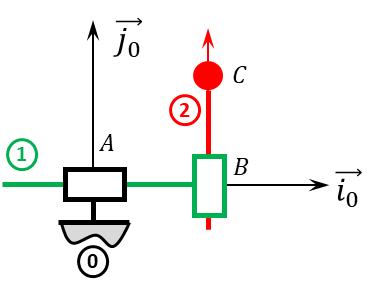
\includegraphics[width=.6\linewidth]{03_TT_01}
\end{center}
\fi

\question{Réaliser le graphe d'analyse en faisant apparaître l'ensemble des actions mécaniques.}
\ifprof
\else
\fi

\question{Donner le torseur de chacune des actions mécaniques.}
\ifprof
\else
\fi


\question{Simplifier les torseurs dans l'hypothèse des problèmes plans.}
\ifprof
\else
\fi

\question{Proposer une démarche permettant de déterminer les efforts que doivent développer chacun des vérins  pour maintenir le mécanisme en équilibre.}
\ifprof
\else
\fi


\ifprof
\else
\begin{flushright}
\footnotesize{Corrigé  voir \ref{C1:05:03}.}
\end{flushright}%
\fi